% coding:utf-8

%----------------------------------------
%FOSADSVB, a LaTeX-Code for a summary of digital signal processing
%Copyright (C) 2015, Mario Felder & Michi Fallegger

%This program is free software; you can redistribute it and/or
%modify it under the terms of the GNU General Public License
%as published by the Free Software Foundation; either version 2
%of the License, or (at your option) any later version.

%This program is distributed in the hope that it will be useful,
%but WITHOUT ANY WARRANTY; without even the implied warranty of
%MERCHANTABILITY or FITNESS FOR A PARTICULAR PURPOSE.  See the
%GNU General Public License for more details.
%----------------------------------------

\chapter{Digitale Signale im Frequenzbereich}
\section{Von Fouriertranformation zur DFT}
\subsection{Übergang zu diskreter Zeit (DTFT)}
Die zeitdiskrete Fourier Transformation (DTFT) berechnet sich mit der normalisierten Winkelfrequenz $\Omega$:
\[ \Omega = 2\pi f T_S = 2\pi\frac{f}{f_S} \left[\frac{rad}{sample}\right] \hspace{35mm} 
X(\Omega) = \sum_{n=-\infty}^{\infty} x[n] \cdot \e^{-\im\Omega n} \]
Die DTFT produziert ein $2\pi$-periodisches, kontinuierliches Spektrum.
Das Mapping sieht wie folgt aus:
\begin{center}
	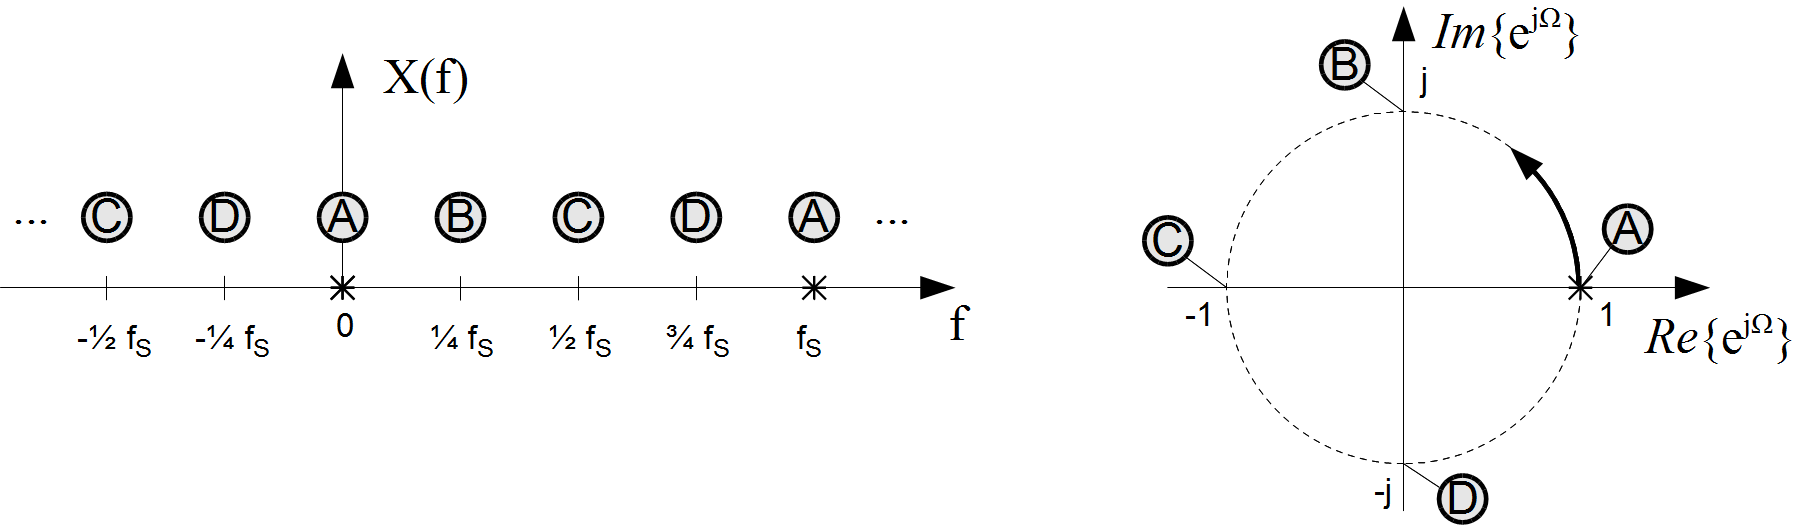
\includegraphics[width=.7\textwidth]{../fig/dtft_frequency_mapping}
\end{center}

%===============================================================================
\subsection{Übergang zu endlichem Messintervall (DFT)}
Je mehr Abtastpunkte bzw. je länger das Messinverval $T$, desto höher die Auflösung. 
Da in der Praxis nur über $N$ Abtastpunkte eine Fourier Analyse gemacht werden kann,
ist die kleinste Frequenzänderung $\Delta f$, welche festgestellt werden kann:
\[ \Delta f = \frac{1}{T} = \frac{1}{N \cdot T_S} = \frac{f_S}{N} \]
Die Diskrete Fourier Transformation (DFT) kann geschrieben werden als:
\[ X[k] = \sum_{n=0}^{N-1}x[n] \cdot e^{-j 2 \pi n \frac{k}{N}} \qquad 
	k = 0,1, 2, \ldots , N-1 \]
Dabei beschreibt $n$ den diskreten Zeitindex, $k$ den diskreten Frequenzindex.\\\\
Die DFT produziert ein diskretes und periodisches Linienspektrum mit Auflösung $f_S/N$. 
Die DFT berechnet die Spektralwerte an den folgenden Frequenzpunkten:
\[ 0,\ \frac{f_S}{N},\ 2\frac{f_S}{N},\ ...,\ (N-1)\frac{f_S}{N} \qquad \mathrm{oder}
 \qquad f_k = k \cdot \frac{f_S}{N} \mathrm{\ mit\ } 0 \leq k \leq N-1\]
Die DFT ist demnach beschränkt zu einer maximalen Frequenz von:
\[ f_{max}=(N-1)\frac{f_S}{N} \]
Die inverse diskrete Fourier Transformation (IDFT) ist gegeben durch:
\[ x[n] = \frac{1}{N} \sum_{k=0}^{N-1} X[k] \cdot e^{j 2\pi n \frac{k}{N}} 
	\qquad n = 0,1, 2, \ldots , N-1 \]
\textbf{Achtung:}
Bei der IDFT wird über die Anzahl Samples normiert, bei der DFT jedoch nicht!
\newpage

%===============================================================================
\subsection{Vergleich der Fourier-Methoden}
Die folgenden Punkte können festgehalten werden:
\begin{itemize}[noitemsep,topsep=3pt]
	\item Periodizität im Zeitbereich resultiert diskretes Linienspektrum im Frequenzbereich.
	\item Sampling im Zeitbereich resultiert in einem periodischen Spektrum.
\end{itemize}
\begin{center}
	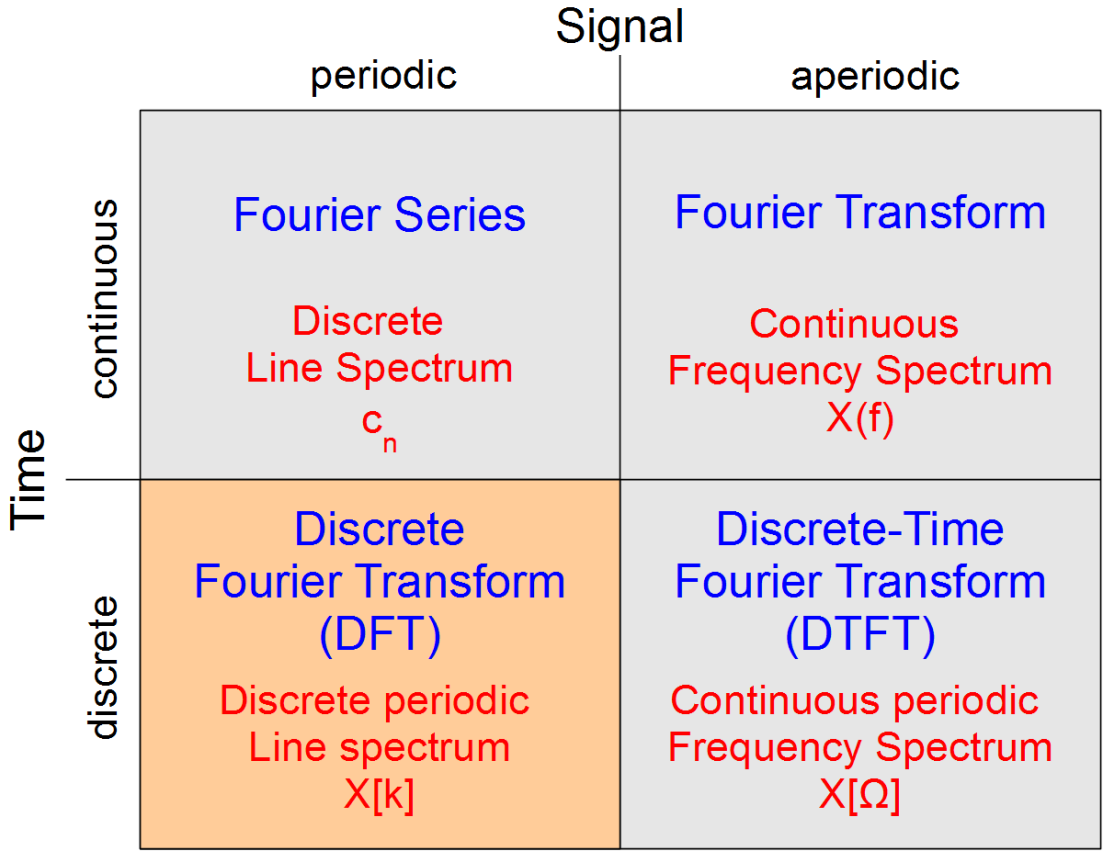
\includegraphics[width=.4\textwidth]{../fig/fft_methods}
\end{center}

%===============================================================================
\subsection{Intuitiver Ansatz zum Verständnis der DFT}
Wendet man auf die Definition der DFT Analyse die eulersche Identität an, 
ergibt sich die Definition in Summen-Form, aufgeteilt in einen Real- und einen 
Imaginäranteil:
\[ X[k]=\underbrace{\sum_{n=0}^{N-1}x[n]\cos(2\pi k\frac{n}{N})}_{\Re\{X[k]\}}
	+ j \cdot \underbrace{\sum_{n=0}^{N-1}x[n](-1)\sin(2\pi k \frac{n}{N})}_
	{\Im\{X[k]\}} \]
Im Endeffekt handelt es sich beim Realanteil des Resultates der DFT $X[k]$ um 
eine statische Korrelation des Signals $x[n]$ mit $cos(2\pi nk/N)$. 
Beim Imaginäranteil von $X[k]$ handelt es sich um eine statische Korrelation 
des Signals $x[n]$ mit $-sin(2\pi nk/N)$. Der Index $k$ gibt dabei an, wie oft die Schwingung in einer Periode platz hat.\\\\
Die folgende Graphik stellt den Zusammenhang graphisch dar für $k=1$ \& $N=16$.
\begin{center}
	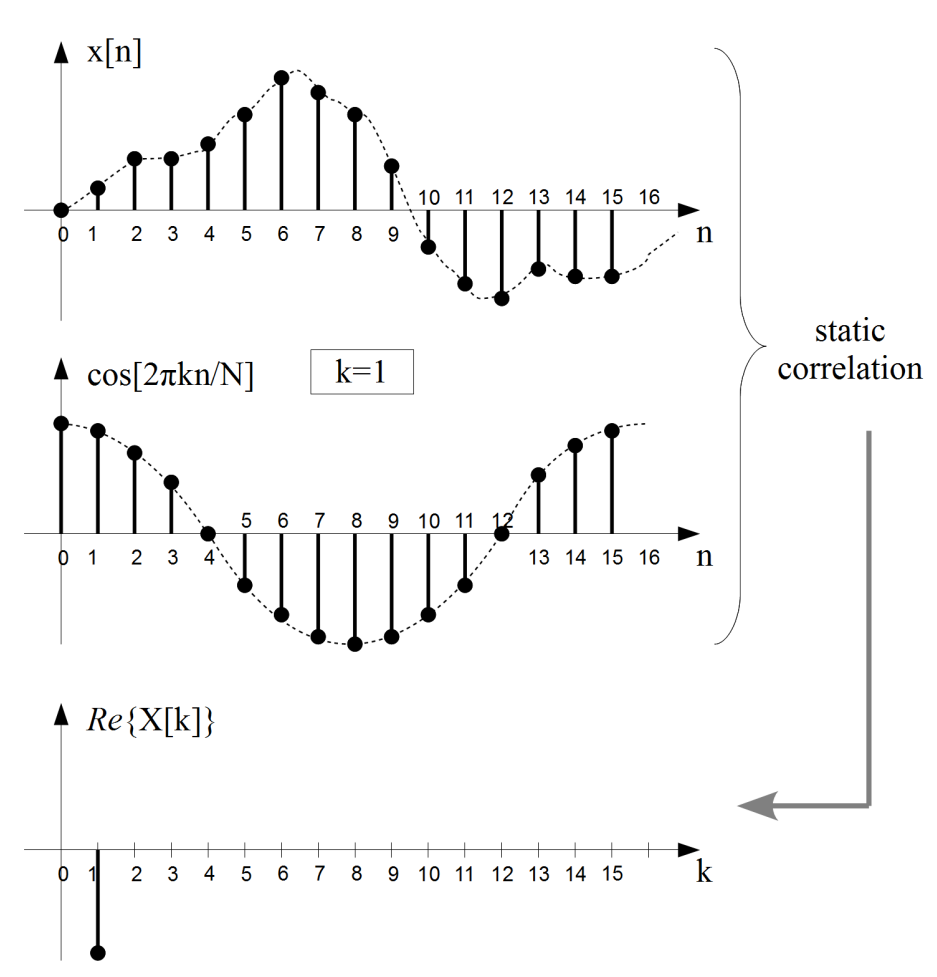
\includegraphics[width=.475\textwidth]{../fig/dft_intuitiv}
\end{center}

%===============================================================================
\section{Eigenschaften der DFT}
\textbf{Periodizität:}
Das Spektrum der DFT ist aufgrund der diskreten Samples $f_S$-periodisch:
\[ X[k] = X[k+N] \]
Das Spektrum wiederholt sich alle $f_S$ Hertz. Für eine Frequenz $f_1$ entsteht Aliasing bei:
\[ f_k = k \cdot f_S \pm f_1 \qquad k= \{1, 2, 3, ...\} \]
Dementsprechend ist IDFT periodisch mit $T=N\cdot T_S$:
\[ x[n] = x[n+N] \]\\
\textbf{Symmetrie:}
Die DFT eines realwertigen Signals ist symmetrisch um den Punkt $k=N/2$:
\[ X[N/2+m] = X^*[N/2-m] \]\\
\textbf{Zeit/Frequenz Verschiebung:} Eine Verschiebung der Sequenz im Zeitbereich um $n_0$ Samples hat einen linearen 
Phasenoffset bei allen Spektralwerten zur Folge. Die zu addierende Phase ist $\varphi=2\pi n_0 \frac{k}{N}$ und muss 
demnach für jedes $k$ berechnet werden. Der Betrag bleibt unverändert.
\[ x[n+n_0] \qquad \laplace \qquad e^{j 2\pi n_0 \frac{k}{N}} \cdot X[k] \]
Die Multiplikation mit einem komplexen Exponent hat eine konstante
Frequenzverschiebung zur Folge:
\[ e^{j 2\pi k_0 \frac{n}{N}} \cdot x[n] \qquad \laplace \qquad X[k-k_0] \]\\
\textbf{Modulation:} Konsequenz der Frequenzverschiebung ist die Modulation:
\[ \cos\left(2\pi k_0\frac{n}{N}\right) \cdot x[n] \qquad\laplace\qquad
	\frac{1}{2}\left( X[k+k_0] + X[k-k_0] \right) \]\\
\textbf{Parseval Theorem:}\\
Zwischen Signalwerten $x[k]$ und Fourier Koeffizienten $X[k]$ besteht folgende
Beziehung. Der linke Teil repräsentiert dabei die durchschnittliche Signalleistung
des Signals $x[n]$. Das Parseval Theorem kann eingesetzt werden, um das SNR mittels 
den Fourier-Koeffizienten $X[k]$ zu bestimmen. Zuerst müssen dazu die Nutzsignal-Frequenzen 
von den Rausch-Frequenzen unterschieden werden.
\[ \frac{1}{N} \sum_{n=0}^{N-1}x[n]^2 = \sum_{k=0}^{N-1}\left| 
	\frac{X[k]}{N} \right|^2  \]\\
\textbf{Zusammenhang von Faltung und Multiplikation:}\\
Punktweise Multiplikation zweier DFT Spektren $X[k]$ und $Y[k]$ im 
Frequenzbereich entspricht der zyklischen Faltung von $x[n]$ und $y[n]$ im 
Zeitbereich:
\[ x[n] \circledast_N y[n] \qquad\laplace\qquad X[k]\cdot Y[k] \]

%===============================================================================
\subsection{Gültigkeitsbereich der DFT}
Wird die DFT mit endlichem $N$ auf nicht-periodische Signale angewendet, 
muss $x[n]$ ausserhalb von $0 \leq n < N$ Null sein. Dann gilt, dass die 
DFT die DTFT an diskreten Punkten der normalisierten Kreisfrequenz $\Omega$ sampelt:
\[ X[k] = X[\Omega]|_{\Omega=2\pi\frac{k}{N}} \]
\textbf{Fall 1: $x[n]$ periodisch}\\ 
Der Messintervall $N\cdot T_S$ ist ein ganzzahliges Vielfaches der Periodendauer
von $x[n]$.\\
\\
\textbf{Fall 2: $x[n]$ aperiodisch}\\
Alle Werte von $x[n]$ ausserhalb des Bereichs $0\leq n<N$ sind Null. Ansonsten 
ergibt sich nur eine Annäherung. In der Praxis wird der Approximations-Fehler 
durch Fenster-Funktionen reduziert.

%===============================================================================
\section{Anwendungs-Aspekte}
\subsection{Fensterlänge \& Leakage}
Wie im vorherigen Unterkapitel (Fall 1) beschrieben, muss das Messintervall ein 
ganzzahliges Vielfaches der Periodendauer von $x[n]$ sein. Da dies in der Praxis nicht 
möglich ist, entsteht sogenanntes Leakage. Der Effekt zeigt sich, indem im Bereich
um die eigentlichen Signalfrequenzen "'verschmiert"' wird. Ohne Leakage (links) und 
mit Leakage (rechts):\\\\
\begin{minipage}{.49\textwidth}
	\begin{center}
		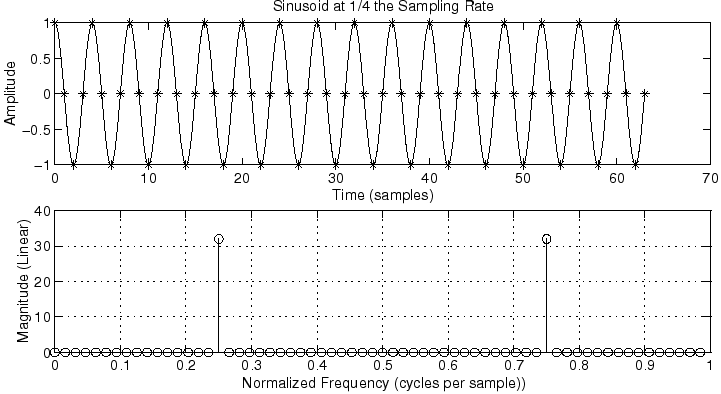
\includegraphics[width=\textwidth]{../fig/dft_no_leakage}
	\end{center}
\end{minipage}
\begin{minipage}{.49\textwidth}
	\begin{center}
		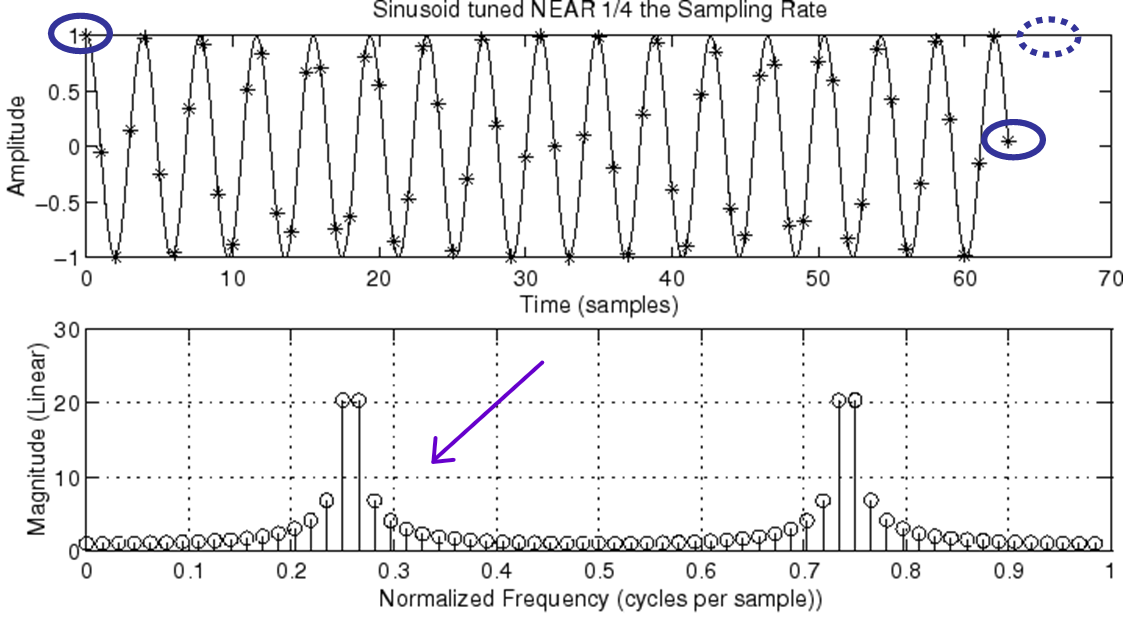
\includegraphics[width=\textwidth]{../fig/dft_leakage}
	\end{center}
\end{minipage}

\subsection{Zero-Padding}
Um eine bessere Interpolation zwischen den $N$ Frequenzpunkten in der DFT zu
bekommen, kann das Signal im Zeitbereich mit Nullen aufgefüllt werden.
Das Spektrum $X(\Omega)$ sowie die Auflösung des Spektrums wird nicht verändert, 
allerdings stehen zusätzliche Abtastpunkte auf der Achse der normalisierten 
Winkelfrequenz $\Omega$ zur Verfügung.

%===============================================================================
\subsection{Fensterfunktion}
Die DFT wendet per Definition ein Rechteckfenster an, um die $N$ Samples
auszuschneiden. Es können andere Fensterfunktionen auf das Signal $x[n]$
angewendet werden, allerdings gelten folgende Punkte:
\begin{itemize}[noitemsep,topsep=3pt]
	\item Je schmaler die Hauptkeule im Spektrum des Fensters, desto höher ist
	die spektrale Auflösung für $X[k]$.
	\item Je stärker die Dämpfung der Nebenkeulen im Spektrum des Fensters, desto
	besser die Unterdrückung der Leakage in $X[k]$.
\end{itemize}

\begin{center}
	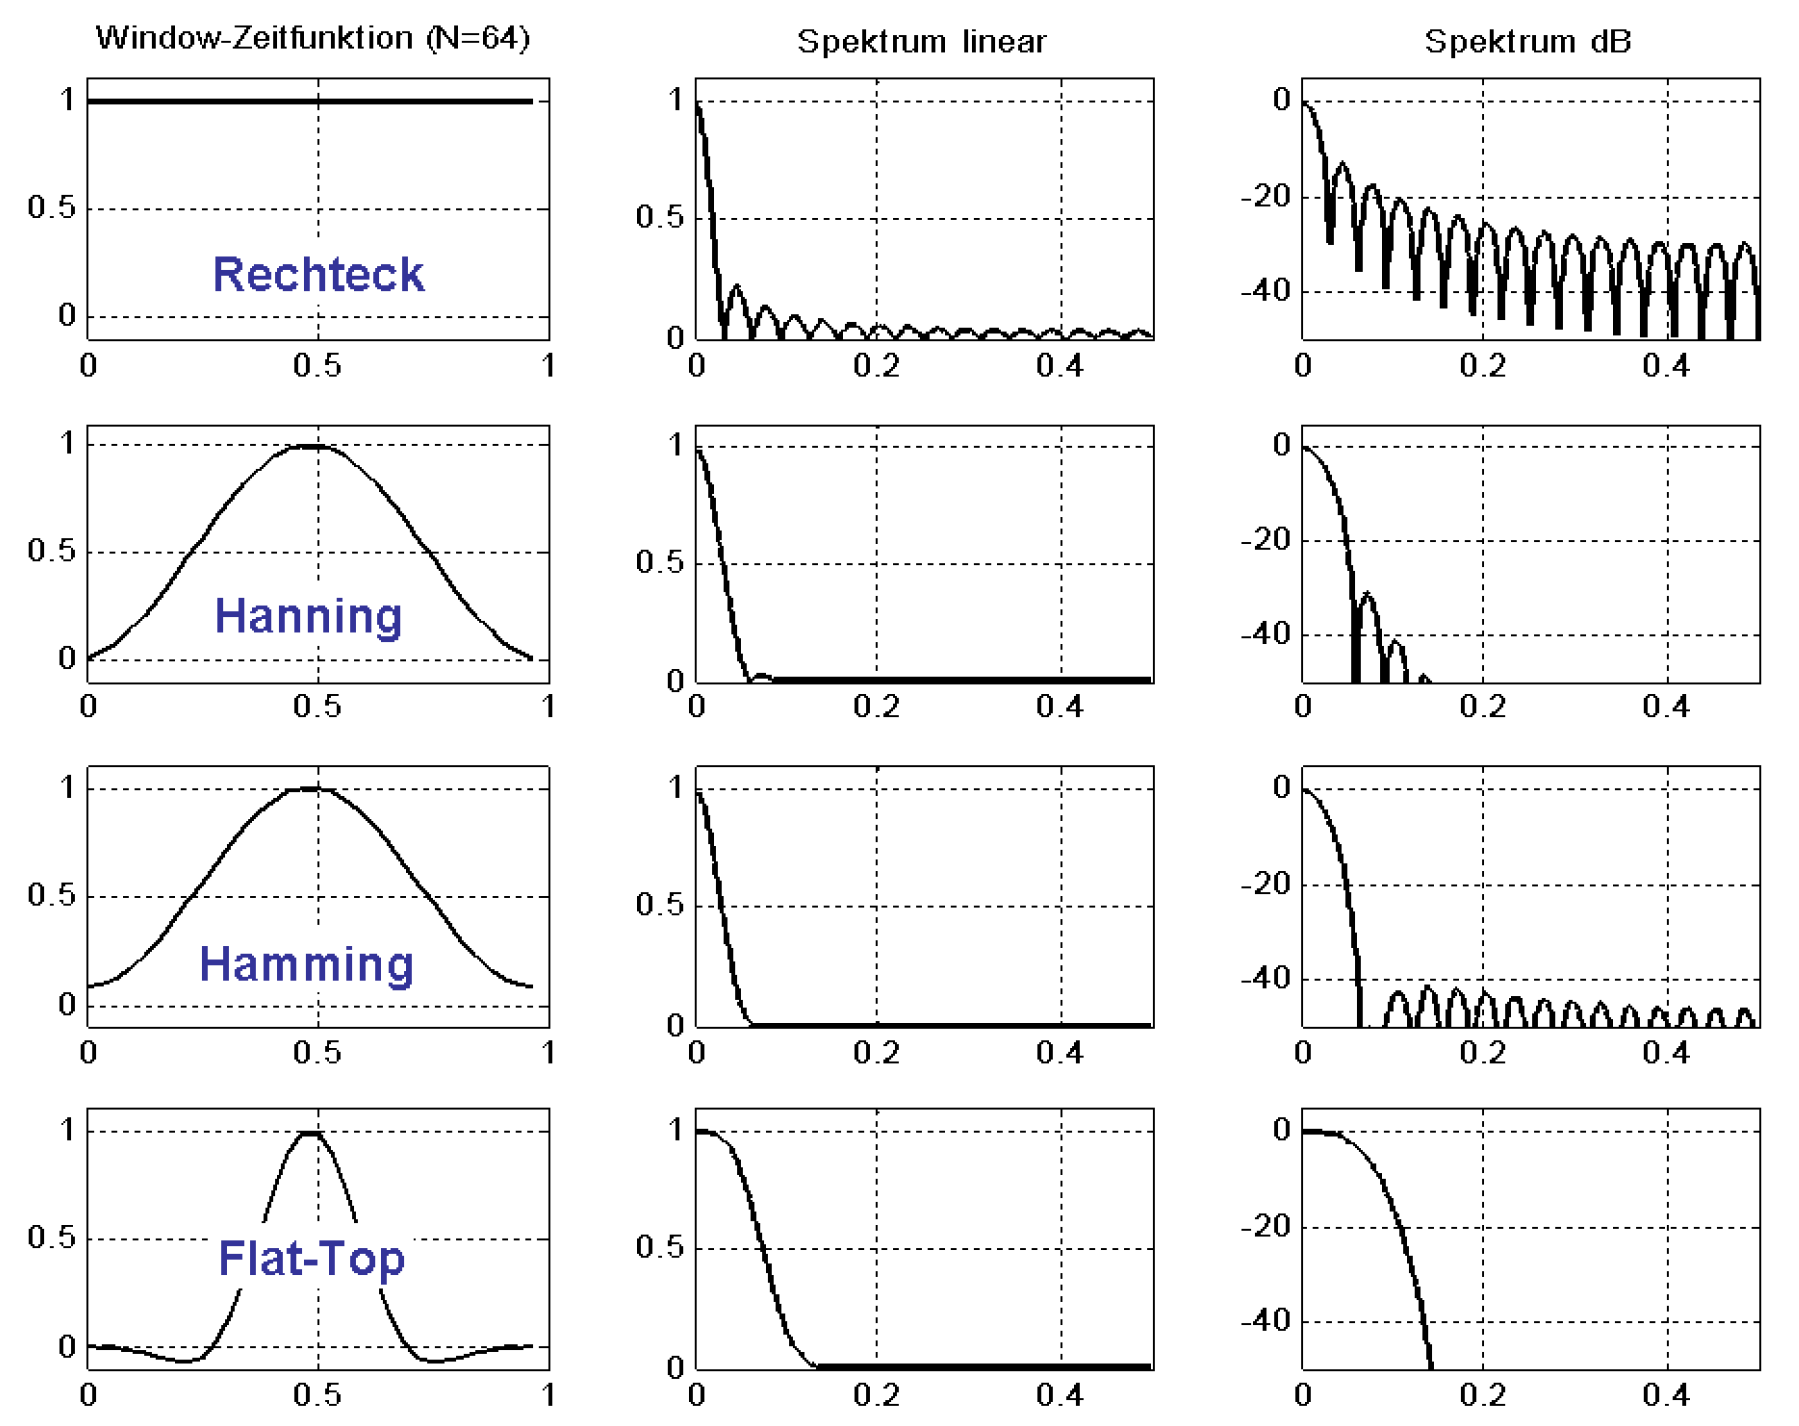
\includegraphics[width=.70\textwidth]{../fig/windows}
\end{center}

%===============================================================================
\section{Short-Time DFT}
Wenn die Entwicklung bzw. der Verlauf des Frequenzspektrums über die Zeit interessiert, werden
kontinuierliche Berechnungen des Spektrums von kurzen Signalsektoren 
durchgeführt. Da diese kurzen Sektoren meistens nicht ein ganzzahliges 
Vielfaches der Periode sind, werden Fensterfunktionen angewendet.\\
\\
Bei der Länge $N$ des Fensters ergibt sich der Kompromiss von:
\begin{itemize}[noitemsep,topsep=3pt]
	\item Grosser spektraler Auflösung ($N$ gross).
	\item Grosser zeitlicher Auflösung ($N$ klein).
\end{itemize}
Um beides zu erreichen, können die DFT-Fenster überlappt werden um maximal
$N-1$.

%===============================================================================
\section{Fast Fourier Transformation (FFT)}
Die FFT ist ein effizienter Algorithmus zur DFT-Berechnung nach dem Teile-und-
Hersche Prinzip. Es wird rekursiv in $r$ Subsequenzen unterteilt. $r$ wird als 
"'radix"' der FFT bezeichnet. Meistens werden radix-2 Algorithmen eingesetzt.\\\\
Die Frequenzauflösung ist gegeben durch, wobei $N = 2^L$ mit einem ganzzahligen Wert für $L$ ist: 
$\Delta f = \frac{f_s}{N}$\\\\
\textbf{Geschwindigkeitsvergleich FFT-DFT:\\}
Vereinfachungen \& Annahmen:
\begin{itemize}[noitemsep,topsep=3pt]
	\item Eine Addition von 2 realen Zahlen ist so rechenintensiv wie eine Multiplikation von 2 realen Zahlen.
	\item Eine komplexe Multiplikation benötigt vier reale Multiplikationen und 2 reale Additionen.
	\item Eine komplexe Addition benötigt zwei reale Additionen.
\end{itemize}
Der speedup factor der FFT ist demnach wie folgt:
\[ \mathrm{speedup\ factor}_{FFT} = \frac{8N-2}{5\cdot \log_2N} \approx 1.5 \cdot	
	\frac{N}{\log_2N} \]
\textbf{Reduktion des Rechenaufwandes:}
\begin{table}[H]
\centering
\begin{tabular}{rl}
Aufwand mit "'normaler"' DFT: & $\left[N^2\right]_\textrm{cpl.Mul.} + \left[N^2-N\right]_\textrm{cpl.Add.}$ \\ 
Aufwand mit FFT: & $\left[\frac{N}{2}\cdot\log_2N\right]_\textrm{cpl.Mul.} + \left[N\cdot\log_2N\right]_\textrm{cpl.Add.}$
\end{tabular}
\end{table}

%===============================================================================
\subsection{Twiddle-Faktoren}
Diese Drehfaktoren werden verwendet, um die Eigenschaften der komplexen Harmonischen
zu beschreiben, mit denen die Korrelation zur Berechnung der DFT im Endeffekt durchgeführt wird. 
Definition:
\[ W_N = \e^{-\im\frac{2\pi}{N}} \]
Die folgenden Eigenschaften werden bei der Anwendung der Twiddle-Faktoren ausgenutzt:\\\\
\textbf{Periodizität:} $W_N$ kann nur für $N$ verschiedene Zahlen ausgewertet werden und ist somit $N$-periodisch:
\[ W_N^{k+N} = W_N^k \]
\textbf{Symmetrie:} Abgesehen vom Vorzeichen nimmt $W_N$ nur $N/2$ verschiedene Werte an:
\[ W_N^{k+N/2} = -W_N^k \]
\begin{center}
	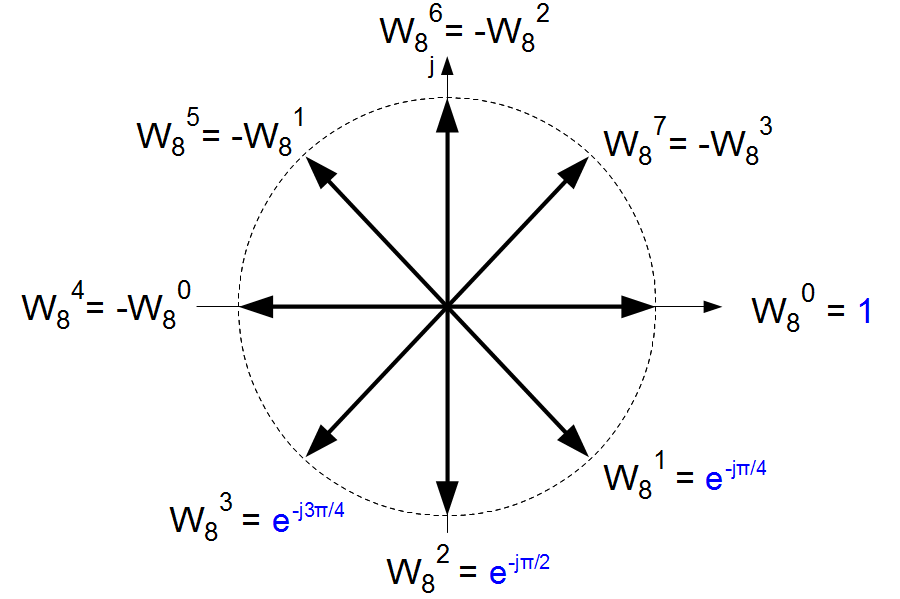
\includegraphics[width=.325\textwidth]{../fig/twiddle_factor}
\end{center}

%===============================================================================
\subsection{Radix-2 FFT}
Die DFT wird mit dem Twiddle Faktor umgeschrieben:
\[ X[k] = \sum_{n=0}^{N-1} x[n] \cdot W_N^{nk}
	= \sum_{n \textrm{ even}} x[n] \cdot W_N^{nk} + \sum_{n\textrm{ odd}}x[n] \cdot W_N^{nk}
\]
Es können zwei neue Sequenzen $x_1[n]$ und $x_2[n]$ mit geraden und ungeraden
$n$ von der Länge $N/2$ erzeugt werden.
\[ X[k] = \underbrace{\sum_{n=0}^{N/2-1}x_1[n] \cdot W_{N/2}^{nk}}_{x_1[\tilde{k}]} +
	W_N^k\cdot \underbrace{\sum_{n=0}^{N/2-1} x_2[n] \cdot W_{N/2}^{nk}}_
	{{x_2[\tilde{k}]}} \hspace{20mm} \mathrm{wobei:} \hspace{2mm} \tilde{k} = k\mod N/2 \]
Im Endeffekt kann die $N$-punkt DFT durch $N/2$ 2-Punkt DTFs ausgedrückt werden. 
Beispiel einer 8-Punkt radix-2 FFT nach Aufteilung in zwei Sequenzen selber Länge (ungerade \& gerade).
Die innere Struktur wird \emph{Butterfly} genannt. Es handelt sich bereits um eine vereinfachte
Struktur der inneren \emph{Butterflys}.
\begin{center}
	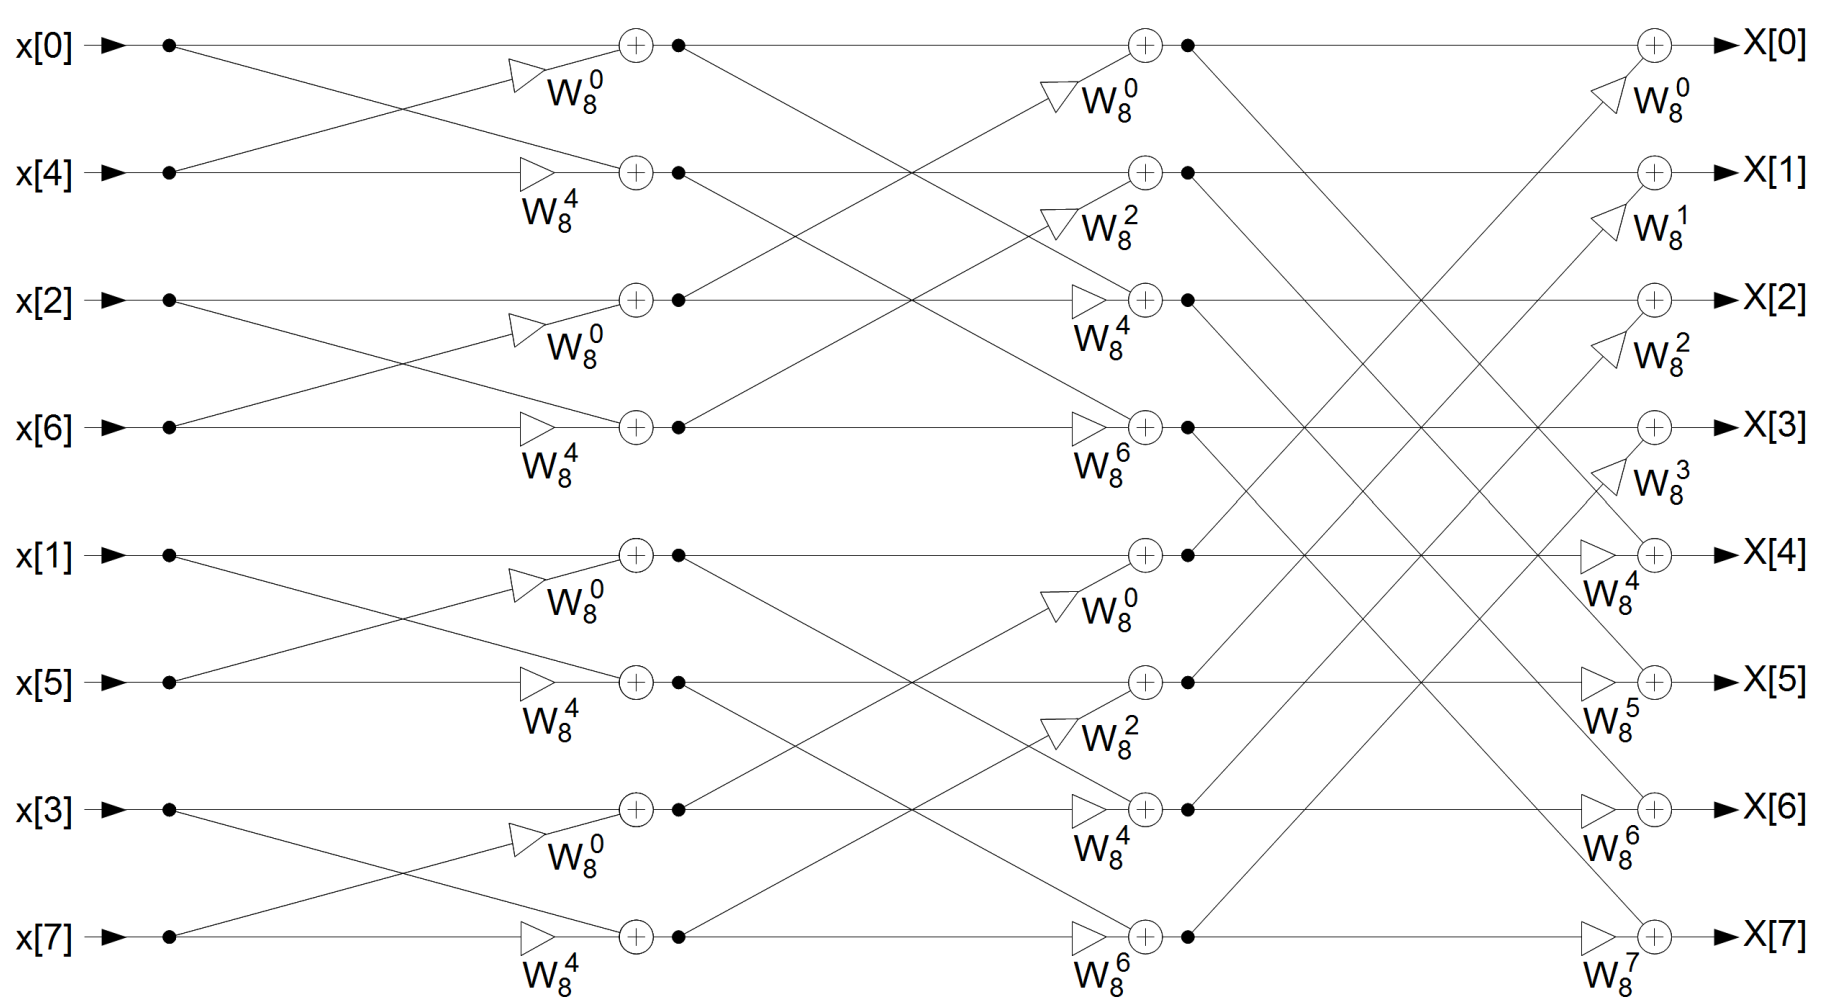
\includegraphics[width=.8\textwidth]{../fig/fft}
\end{center}
Benötigter Speicher der FFT bei in-place (speicheroptimiert): $2N$ ($N$ komplexwertige Koeffizienten) + $N$ ($N/2$ komplexwertige Twiddle Faktoren)\\
Index bit-reversed in Matlab: \verb|bitrevorder()|\\\\
Matlab-Befehle für Darstellung des Spektrum eines Signals \verb|x1|:\\
\verb|n = length(x1); % # of samples in x1|\\
\verb|plot([-n/2:1:n/2-1],20*log10(abs(fftshift(fft(x1)))));|\\
\verb|axis([-1e4 1e4 -200 0]); grid on;|\\
\verb|ylabel('X_1(f)_{dB}'); title('\bf{Original Spectra}');|\\
\begin{center}
	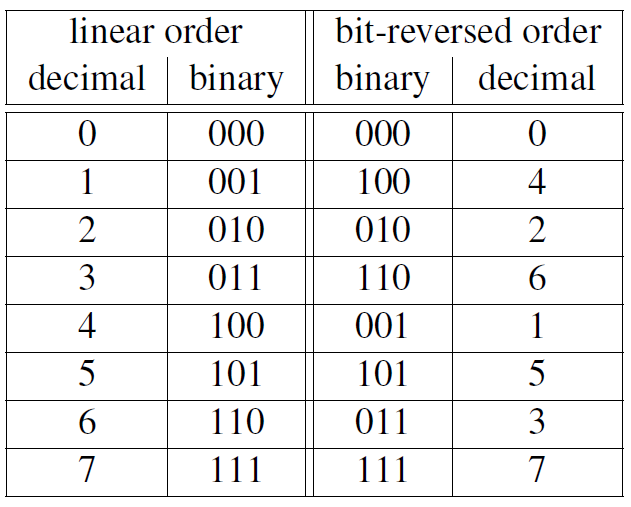
\includegraphics[width=.3\textwidth]{../fig/bit_reversed_order}
\end{center}
\newpage

%===============================================================================
\section{Goertzel-Algorithmus}
Der Goertzel Algorithmus beschreibt einen anderen Ansatz zur DFT-Berechnung mittels linearer Filtertechnik. Er dient dazu, eine bestimmte Frequenzkomponenten $X[k]$ aus den $N$ möglichen Komponenten zu berechnen. Definition:
\[ X[k] = y_k[n]|_{n=N} = \sum_{i=0}^{N-1}x[i] \cdot W_N^{-k(N-i)} \]
Übertragungsfunktion des Filters:
\[H_k(z) = \frac{1}{1-W_N^{-k}z^{-1}} \]
Differenzengleichung:
\[ s[n] = x[n] + a \cdot s[n-1] - s[n-2] \]
\[ y_k[n] = s[n] - W_N^k \cdot s[n-1] \]
mit 
\[ a= 2\cos 2\pi\frac{k}{N} \]
$s[n]$ muss für alle Zeitpunkte $n=0,1,\ldots,N$ berechnet werden, $y_k[n]$
nur für $n=N$ (unten gestrichelt).

\begin{center}
	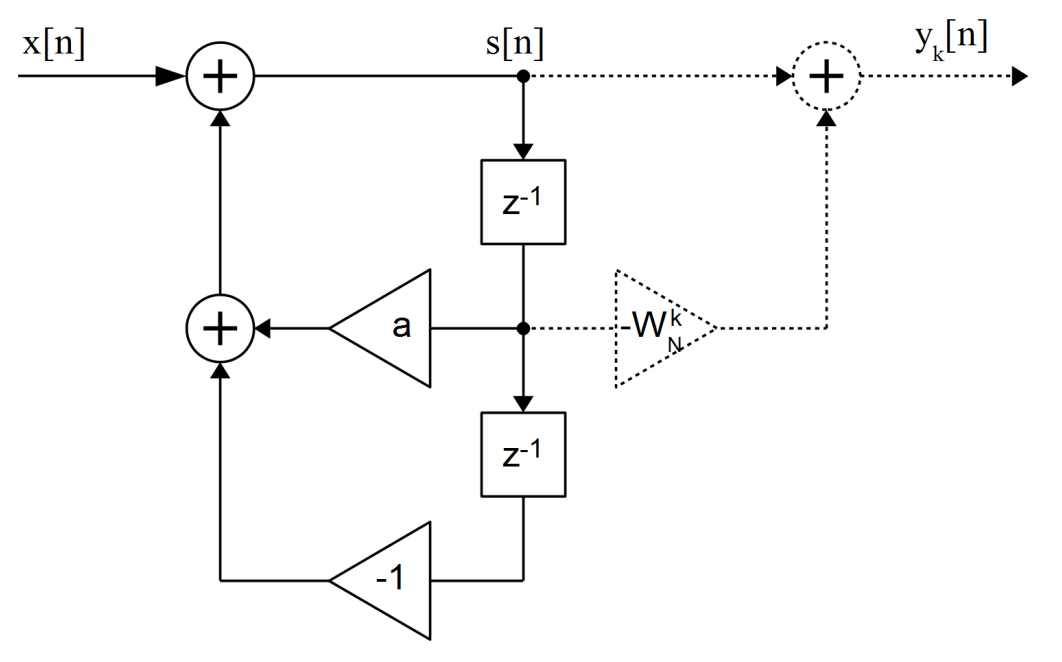
\includegraphics[width=.45\textwidth]{../fig/goertzel}
\end{center}
Der Goertzel-Algorithmus ergibt die DFT Spektralkomponente bei der Frequenz:
\[ f_k = k\frac{f_S}{N} \]
Mit dem Parseval Theorem kann der Leistungsgehalt $P_k$ eines realwertigen
Signals $x[n]$ bei einer Frequenz von $f_k$ ermittelt werden:
\[
	P_k = 2\left| \frac{X[k]}{N} \right|^2
		= \frac{2}{N^2}(\Re\{X[k]\}^2+\Im\{X[k]\}^2)
\]
~\\
\textbf{Rechenaufwand: }
Für reelle Eingangssignale $x[k]$ benötigt der Algorithmus für die Spektrumskomponente 
(positive und negative) dabei $N+1$ reale Multiplikationen und eine komplexe Multiplikation.